\newpage
\section*{Agustinus Adisutjipto: Bapak Penerbang Indonesia}

\begin{floatingfigure}[l]{2cm}
\begin{center}
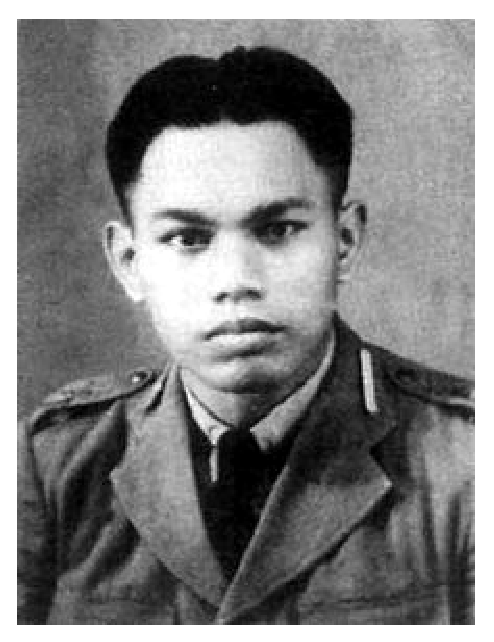
\includegraphics[scale=0.25]{Adisutjipto.ps}
\end{center}
\end{floatingfigure}
Lahir di Salatiga, Jawa Tengah, 3 Juli 1916 - meninggal di Bantul, Yogyakarta 29 Juli 1947 pada umur 31 tahun. Beliau adalah seorang Katolik, pahlawan nasional, dan seorang komodor udara Indonesia

Agustinus Adisutjipto sempat belajar di Sekolah Tinggi Kedokteran (Geneeskundige Hoge School) di Jakarta, tetapi tidak selesai. Kemudian ia memutuskan untuk pindah ke Sekolah Penerbang Militaire Luchtvaart di Kalijati. Selesai pendidikan ia bertugas di Squadron Pengintai Udara.

Sesudah Indonesia merdeka, ia menyumbangkan tenaga membina Angkatan Udara Republik Indonesia bersama S. Suryadarma, yang kemudian diangkat menjadi Kepala Staf AURI. Saat itu, tenaga penerbang sangat sedikit. Pesawat terbang hampir-hampir tidak ada, dan kalau pun ada sudah rongsokan. Teknisi-teknisi Indonesia berusaha memperbaiki pesawat tersebut. Tanggal 27 Oktober 1945, Adisutjipto berhasil menerbangkan sebuah pesawat. Penerbangan itu adalah penerbangan pertama yang dilakukan oleh putra Indonesia. Pada tanggal 1 Desember 1945 Adisutjipto mendirikan Sekolah Penerbang di Yogyakarta, tepatnya di Lapangan Udara Maguwo, yang kemudian diganti namanya menjadi Bandara Adisucipto, untuk mengenang jasa beliau sebagai pahlawan nasional. Di situ dididik kader-kader Angkatan Udara. Karena jasa-jasanya itu Adisutjipto disebut bapak Penerbang Indonesia.

Jabatan lain yang pernah dipegangnya ialah Wakil II Kepala Staf Angkatan Udara. Selain itu, pernah pula ditugasi ke India dan Filipina untuk mencari tenaga pelatih dan menyewa pesawat terbang. Di India, berkat bantuan Perdana Menteri Jawaharlal Nehru, ia berhasil mengadakan perundingan dengan Patnaik yang kemudian bersedia menyewakan sebuat pesawat Dakota.

Agustinus Adisutjipto adalah pribadi yang mempunyai komitmen tinggi terhadap negara dan bangsa. Komitmen itu tidak lepas dari hidup imannya yang kuat. Iman kepada Kristus telah menggerakkan hidupnya untuk melayani dan mengabdi kepada sesama bangsa dan negara meski risiko besar harus ditanggung.

{\small Marsekal Muda (Pur) Agustinus Adisutjipto akrab dipanggil Cip namun kemudian rekan-rekannya memanggilnya Pak Adi merupakan putra pertama dari lima bersaudara buah perkawinan Roewidodarmo dan Latifatun. Adisutjipto, sangat gemar bermain sepakbola, naik gunung, tenis dan catur. Intelektualitasnya terasah lewat hobinya membaca buku-buku kemiliteran dan filsafat. Pribadinya dikenal pendiam, namun sangat reaktif bila harga dirinya terinjak. Ketika Jepang mendarat Maret 1942, peta penerbangan Hindia Belanda berubah. Adisutjipto yang ketika PD II pecah ditempatkan di skadron intai di Jawa beserta rekan-rekannya seperti Sujono, Sulistyo, dan Husein Sastranegara, tidak pernah lagi terbang. Semua yang berbau Belanda dimusnahkan. Untuk mengisi kekosongan, Cip bekerja di perusahaan angkutan bus milik Jepang.

Sejak pekik kemerdekaan berkumandang 17 Agustus 1945, satu demi satu muncul berbagai tuntutan. Termasuk penerbangan militer. Suryadarma bertindak cepat. Para eks penerbang AU Hindia Belanda, seperti Adisutjipto, dipanggilnya. Berbagai langkah konsolidasi, mulai dari mengumpulkan ratusan pesawat sampai mengupayakan perbaikan pesa-wat-pesawat peninggalan Jepang, diambil.

Usaha Suryadarma langsung berbuah. Buktinya, Adisutjipto berhasil menerbangkan pesawat Nishikoren dari Cibereum ke Maguwo, 10 Oktober 1945. Peristiwa ini tercatat sebagai penerbangan pertama di wilayah RI merdeka oleh awak Indonesia. Tujuhbelas hari kemudian, kembali Adisutjipto membakar semangat perjuangan dengan menerbangkan pesawat Cureng bertanda merah putih. Peristiwa ini mengukir lagi catatan sejarah, sebagai penerbangan berbendera merah putih pertama di tanah air.

Adi Sutjipto terbang ke India untuk mengambil obat2an dan sekembalinya dari India ketika memasuki wilayah Indonesia. Di ujung cakrawala, terlihat pesawat Dakota VT-CLA melakukan approach. Para penumpangnya, Adisutjipto, Abdulrachman Saleh, AN Constantine (pilot), R Hazelhurst (ko-pilot), Adisumarmo Wiryokusumo (engineer), Bhida Ram, Nyonya Constantine, Zainal Arifin (wakil dagang RI), dan Gani Handonocokro, tentu bahagia karena sesaat lagi akan mendarat. Begitu juga Sudarjono yang lagi piket, akan bertemu dengan kakaknya.

Sekonyong-konyong, muncul dua pesawat P-40 Kitty Hawk Belanda dari arah utara yang langsung memberondong Dakota, pesawat sipil yang jelas-jelas membawa bantuan. Pesawat kehilangan ketinggian, melayang kencang dan menyambar sebatang pohon hingga badannya patah menjadi dua bagian. Begitu pesawat terhempas ke tanah, langsung terbakar. Suryadarma dan semua orang penunggu, berlarian ke arah pesawat naas.
Peristiwa itu terjadi di Dusun Ngoto pada tanggal 29 Juli 1947. Beliau dimakamkan di pemakaman umum Kuncen I dan II, dan kemudian pada tanggal 14 Juli 2000 dipindahkan ke Monumen Perjuangan di Desa Ngoto, Bantul, Yogyakarta.
}
\newpage
\section*{Laksamana Madya Yosaphat Sudarso: Berkorban untuk keselamatan teman} 

\begin{floatingfigure}[r]{2cm}
\begin{center}
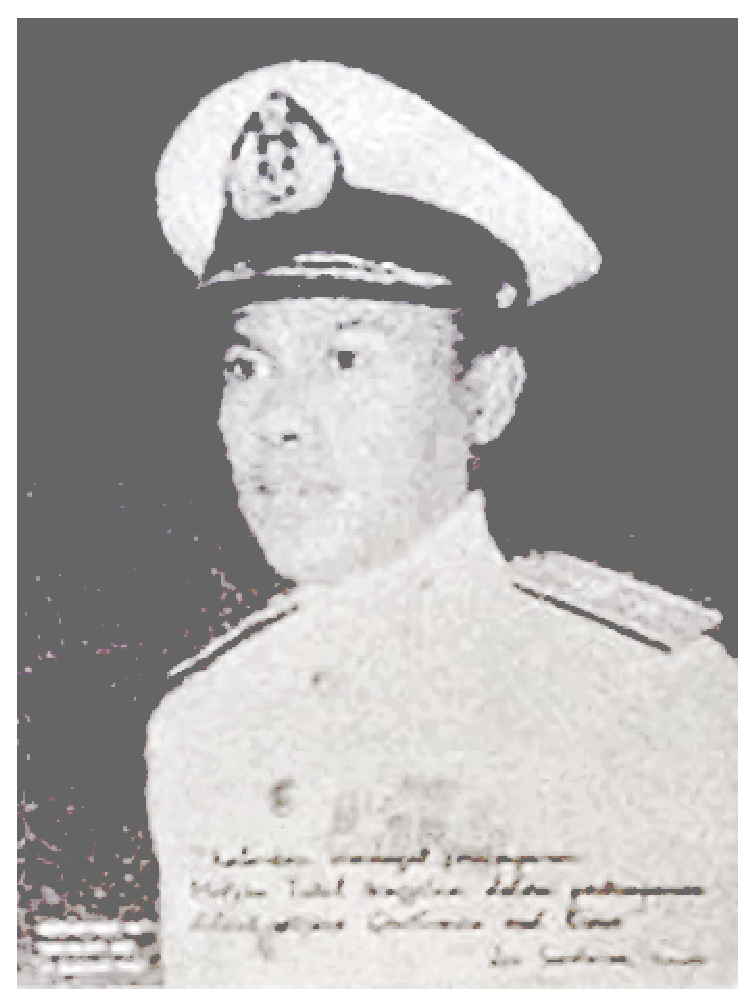
\includegraphics[scale=0.175]{Yos-Sudarso.ps}
\end{center}
\end{floatingfigure}
Laksamana Madya Yosaphat Soedarso atau yang lebih dikenal dengan nama Yos  Sudarso adalah pahlawan nasional Indonesia yang dilahirkan di Salatiga, Jawa  Tengah, 24 November 1925 dan pernah menjabat sebagai Kepala Staff Angkatan Laut.  Meski sebagai orang nomor satu di TNI AL, ia bukanlah tipe pemimpin yang berdiam diri di belakang meja.  Di usianya yang masih muda 36 tahun, ia turut ke medan tempur maju ke garis depan untuk merebut Irian Barat dari kolonial Belanda. Di atas KRI Macan Tutul di Laut Aru, Yos Sudarso gugur dengan berani.

Pertempuran Laut Aru adalah suatu pertempuran yang terjadi di Laut Aru, Maluku, pada tanggal 15 Januari 1962 antara Indonesia dan Belanda. Insiden ini terjadi sewaktu dua kapal jenis destroyer, pesawat jenis Neptune dan Frely milik Belanda menyerang KRI Macan Tutul, KRI Macan Kumbang dan KRI Harimau milik Indonesia yang sedang berpatroli pada posisi 04,49° LS dan 135,02° BT. Komodor Yos Sudarso gugur pada pertempuran ini setelah menyerukan pesan terakhirnya yang terkenal, "Kobarkan semangat pertempuran".

Pada saat itu terjadi pertempuran sengit antara pasukan militer Indonesia  dengan Belanda. Meski berstatus sebagai Kepala Staff TNI-AL Yos sudarso ikut  turut ke medan tempur. Naas dalam peristiwa tersebut, Laksamana Madya Yos  Sudarso gugur setelah KRI Macan Tutul di bombardir Belanda di Laut Aru saat  melawan armada Belanda.

Armada Indonesia di bawah pimpinan Yos Sudarso, yang saat itu berada di KRI Macan Tutul, berhasil melakukan manuver untuk mengalihkan perhatian musuh sehingga hanya memusatkan penyerangan ke KRI Macan Tutul. KRI Macan Tutul tenggelam beserta awaknya, tapi kedua kapal lainnya berhasil selamat.

Beliau gugur di atas KRI Macan Tutul dalam pertempuran Laut Aru pada masa kampanye Trikora. Namanya kini diabadikan pada sebuah KRI dan pulau. Ia gugur di atas KRI Macan Tutul pada tanggal 13 Januari  1962 pada saat berusia 36 tahun. Keikutsertaannya dalam posisi sebagai KSAL-pun  dipertanyakan karena tidak lazimnya seorang Kepala Staff Angkatan Laut turun  langsung dalam medan tempur.

Untuk menghargai jasa-jasa atas keikutsertaannya dalam memperjuangkan merebut Irian  Barat, ia dianugerahi sebagai Pahlawan Pembela Kemerdekaan. Kini namanya  diabadikan sebagai nama armada angkatan laut Indonesia, nama pulau, dan nama  jalan-jalan protokol di kota-kota besar Indonesia.

Ia meninggalkan seorang istri bernama Ny. Siti Kustini, yang dinikahinya pada  tahun 1955 dan dikaruniai lima anak dan dua diantaranya meninggal dunia.

Berselang 44 tahun setelah Yos Sudarso meninggal. Istri pahlawan Aru ini, Nyonya Josephine F Siti Kustini kemudian meninggal. Siti Kustini yang merupakan kelahiran Ngawi, Jawa  Timur, 1935, meninggal dunia pada usia 71 tahun tepatnya, Sabtu 2 September  2006 pukul 14.00, di Rumah Sakit Angkatan Laut Dr Mintohardjo, Jakarta. Akibat penyakit jantung dan radang paru-paru. Jenazah  kemudian dimakamkan, Senin, 4 September 2006 di Tempat Pemakaman Umum Kaliwuluh,  Desa Kaliwuluh, Kecamatan Kebak Kramat, Kabupaten Karanganyar, Jawa Tengah.

Semasa hidupnya, Ny. Siti Kustini dikenal sebagai orang yang sangat disiplin, selalu tepat  waktu, termasuk menunaikan ibadah agama dengan mengikuti misa kudus hampir  setiap hari.

Sebelum pemberangkatan jenazah dari Jakarta menuju Surakarta dengan menggunakan pesawat TNI AL dari Bandar Udara Halim Perdanakusuma. Misa arwah terlebih dahulu dilakukan yang dipimpin Pastor Luarens di kediaman almarhumah, di jalan  Cimandiri Nomor 12, Cikini, Jakarta Pusat. Saat itu juga dihadiri mantan Kepala  Staf TNI Angkatan Laut Laksamana (Purn) Sudomo, mantan Gubernur DKI Jakarta Ali  Sadikin, dan sesepuh TNI AL lainnya



